
\begin{SCfigure*}[][p]
	\centering
	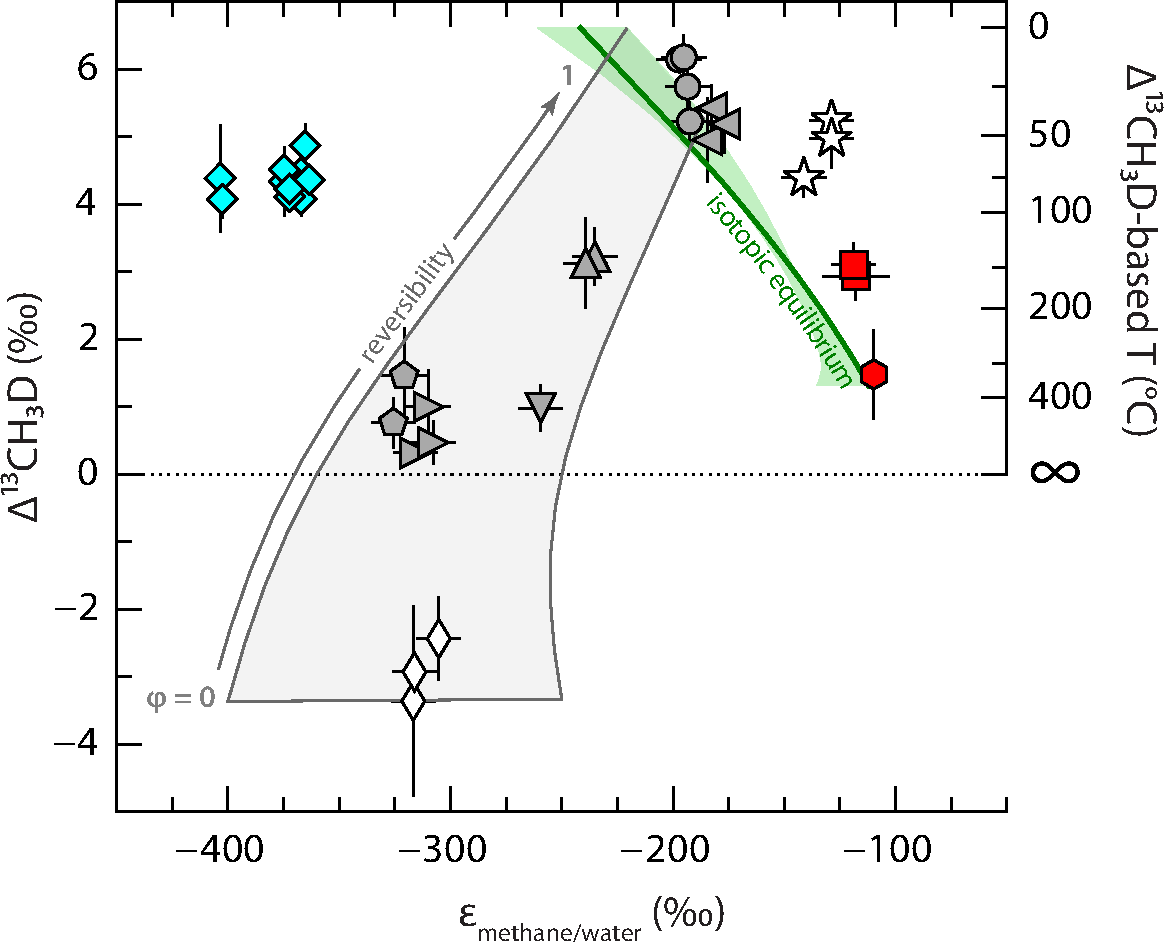
\includegraphics[width=0.5\linewidth]{figures/Fig2.2}
	\caption[Extent of clumped- and hydrogen-isotopic disequilibria in methane]{Extent of clumped- and hydrogen-isotopic disequilibria in methane. Symbols and vertical error bars are the same as those in \autoref{fig:2:1}.
	Horizontal error bars represent uncertainties on estimates of
	$\varepsilon$\textsubscript{methane/water}\footref{fn:2:epsilon} (\autoref{tab:2:S4}). The solid
	green curve represents isotopic equilibrium, with the
	$\varepsilon$\textsubscript{methane/water} calibration given by \textcite{Horibe+Craig_1995_GCA}. Green
	shading represents ranges of $\varepsilon$\textsubscript{methane/water} calibrations
	from published reports (\autoref{fig:2:S3}). Gray shading represents model
	predictions from this study for microbial methane formed between 0 and
	40~°C. Metabolic reversibility ($\varphi$) increases from bottom ($\varphi$ = 0,
	fully-kinetic) to top ($\varphi$ → 1, equilibrium) within this field
	(see \autoref{model-of-isotopologue-systematics-during-microbial-methanogenesis}).}
	\label{fig:2:2}
\end{SCfigure*}
